\chapter*{مقدمه}
هدف از این پروژه طراحی کنترل‌کننده برای سیستم
\lr{Ball and Beam}
است.
 این وسیله از معروف‌ترین و ساده‌ترین سیستم‌های کنترل است. این سیستم شامل یک تیر بلند است که قابلیت حرکت توپ داخل آن را دارد. هدف کنترلی در این سیستم، کنترل مکان توپ دقیقا در وسط تیر است. به این منظور  یک سنسور التراسونیک برای تشخیص مکان و سرعت توپ در هر لحظه و یک سروو موتور در وسط یا اطراف تیر برای تولید حرکت دورانی در تیر و کنترل مکان توپ تعبیه شده است. شمای کلی این دستگاه در شکل
\ref{ballbeam}
آورده شده است.
 \begin{figure}[H]
	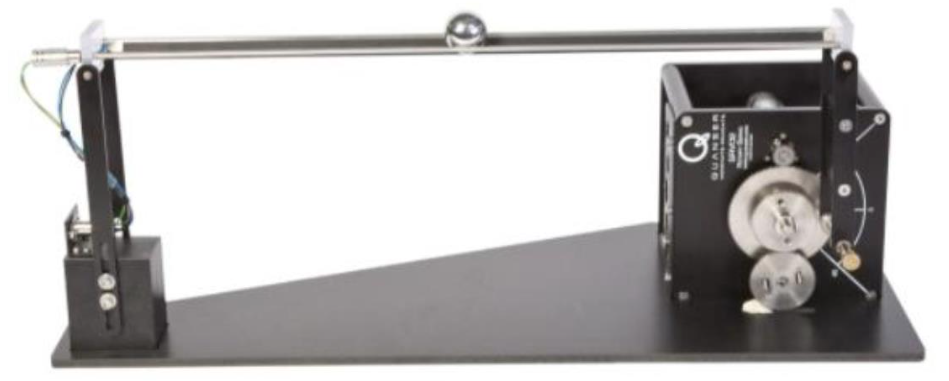
\includegraphics[width=12cm]{../Figure/Introduction/BallBeam.png}
	\centering
	\caption{سیستم کنترلی}
	\label{ballbeam}
\end{figure}
\section*{همکاری}
در پروژه جهت همکاری بین اعضای گروه از گیت هاب استفاده شد که کار را به شدت آسان کرد. در این پروژه تمامی کدها به هم اتصال دارند و با تغییر شرایط اولیه تمامی طراحی‌ها برای سیستم جدید اجرا می‌شوند.
\section*{کنترل‌کننده پایدارساز}
در این پروژه برای پایدار سازی سیستم از کنترل‌کننده \lr{LQG\LTRfootnote{Linear Quadratic Gaussian}} استفاده شد. در شکل
\ref{stabilizer}
خروحی پله حلقه بسته سیستم با کنترل‌کننده پایدار ساز آورده شده است.
 \begin{figure}[H]
	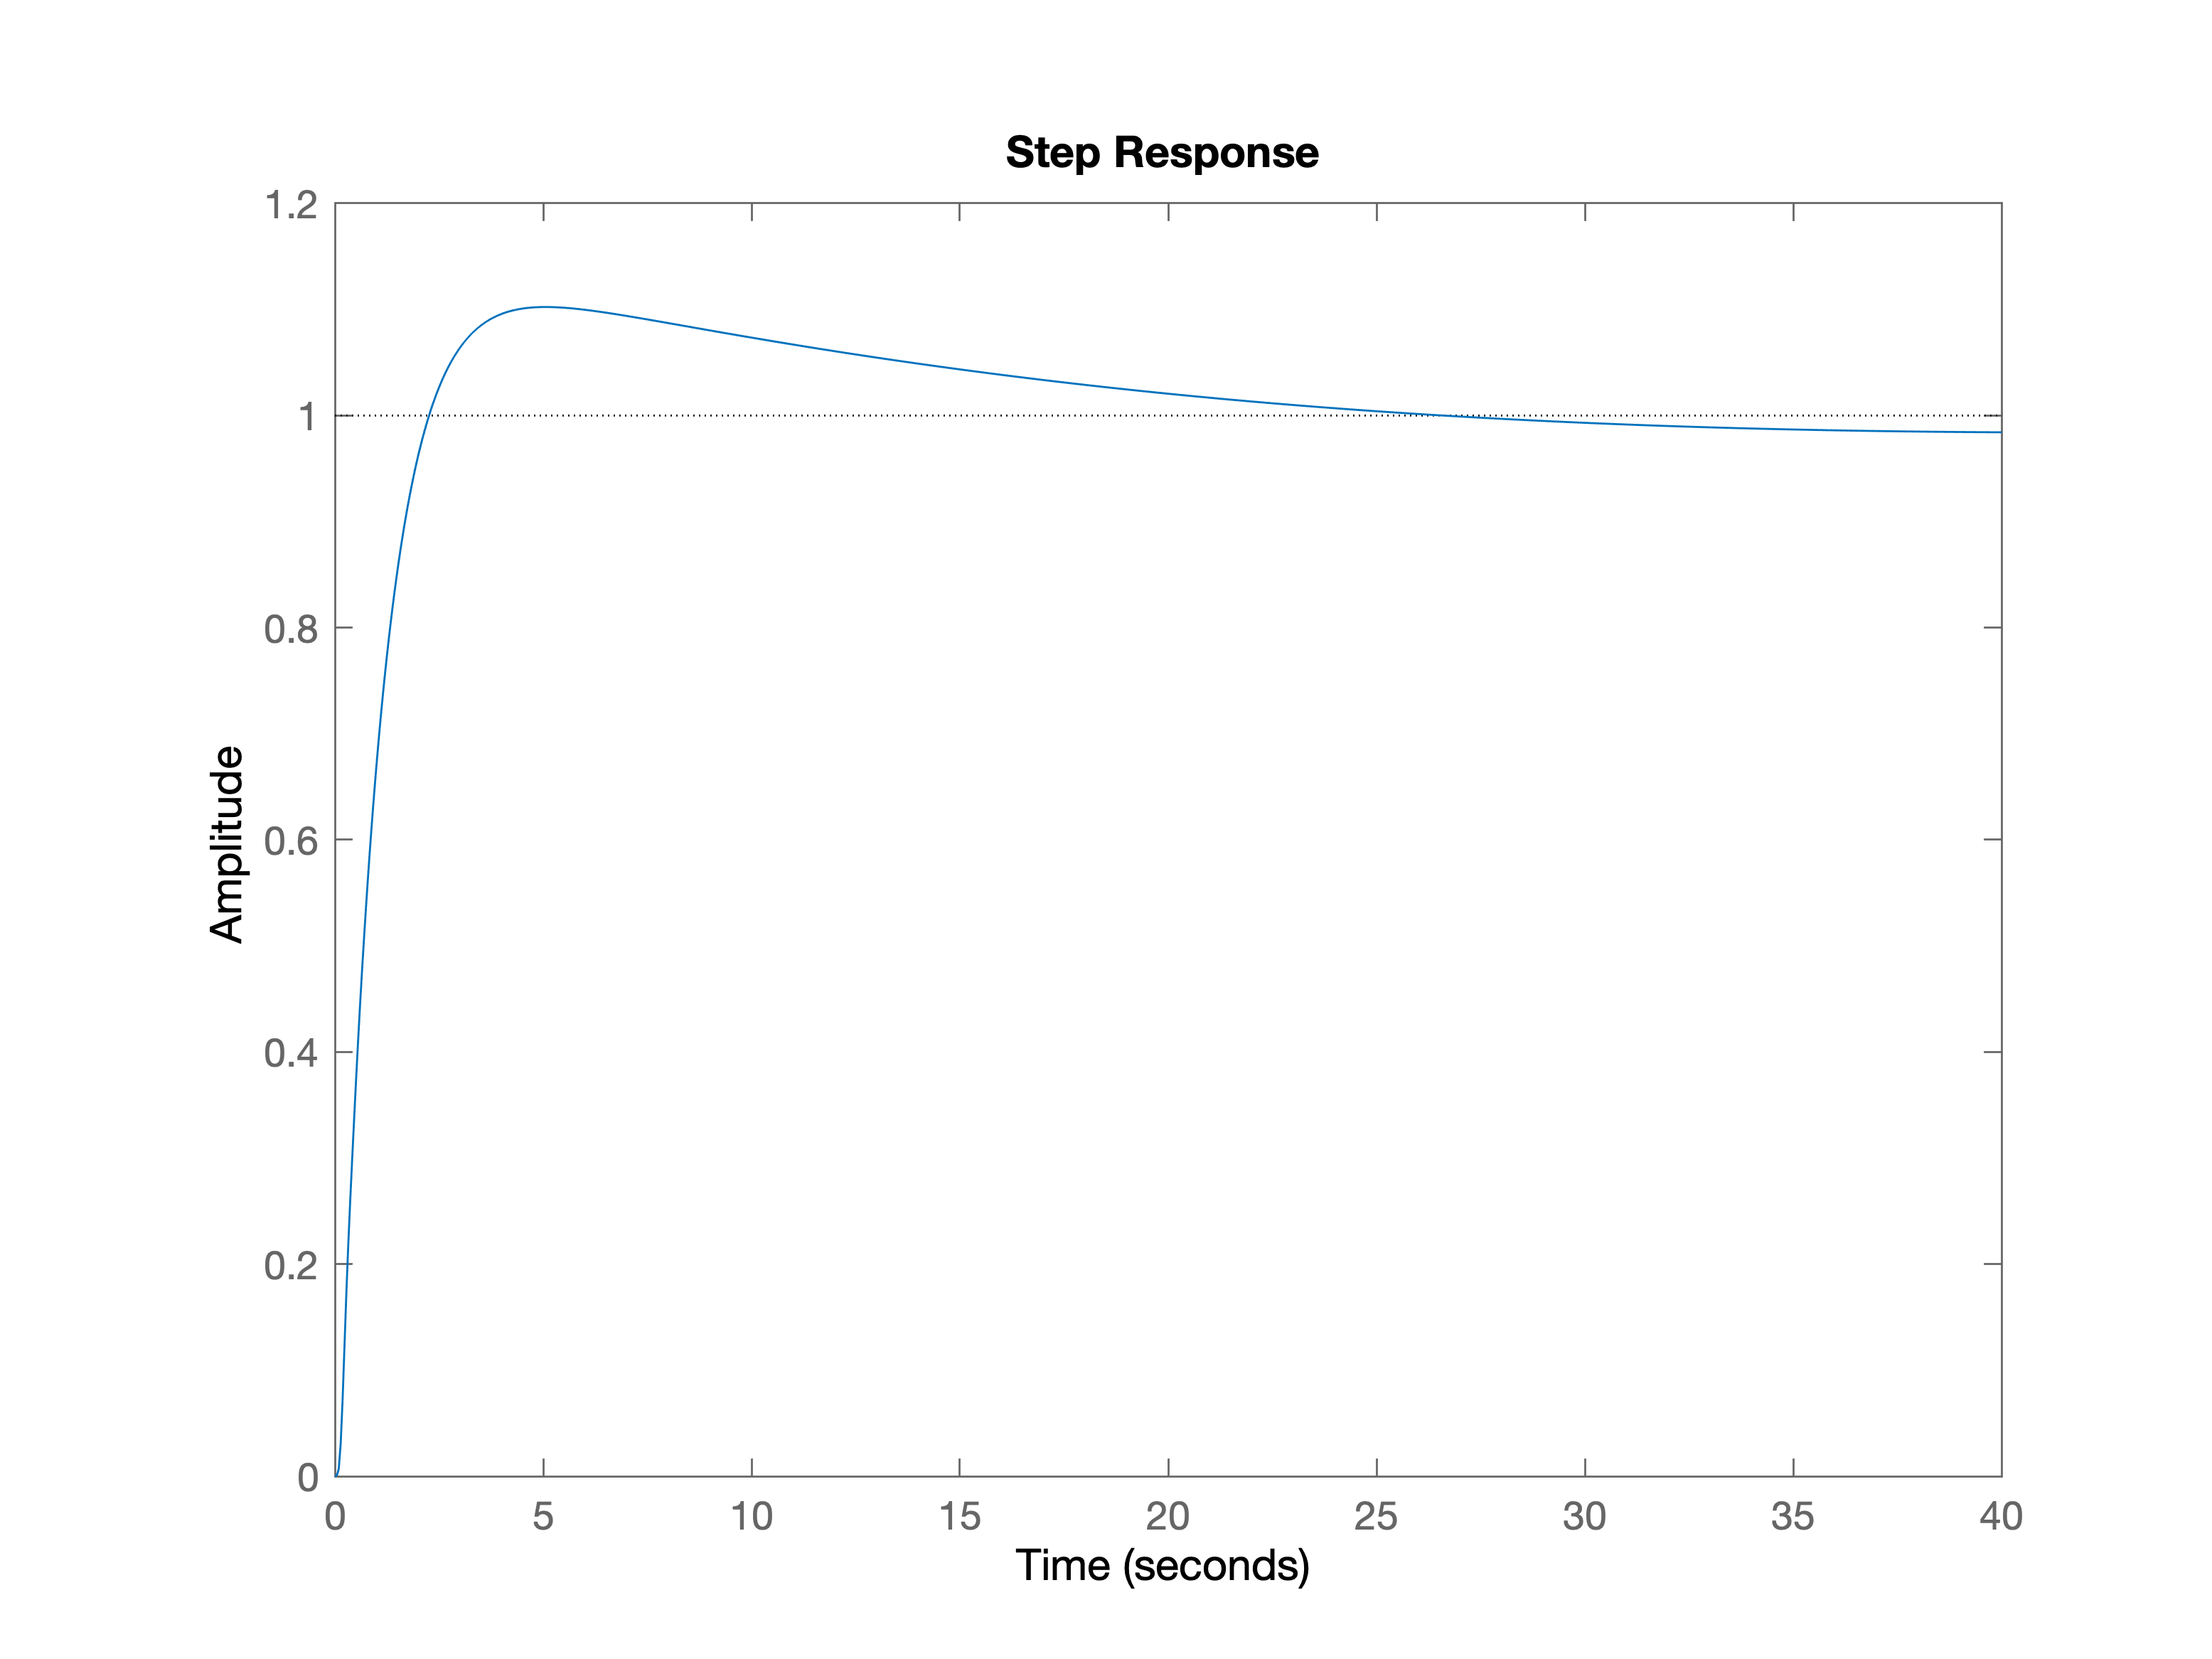
\includegraphics[width=12cm]{../Figure/Introduction/stabilizer.png}
	\centering
	\caption{پله واحد سیستم حلقه بسته در حضور کنترل‌کننده}
	\label{stabilizer}
\end{figure}